De verschillende soorten VPNs op basis van de functionaliteit:
\begin{description}
	\item[site-to-site] is een techniek waarbij twee lokale netwerken (LAN) aan elkaar geknoopt worden via een publiek netwerk (WAN). Zie \ref{fig:VPNSiteToSite}.
	\begin{figure}[h]
	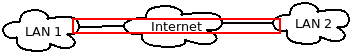
\includegraphics[width=0.9\linewidth]{vpn-site_to_site.png}
	\caption{Site to Site VPN}
	\label{fig:VPNSiteToSite}
	\end{figure}
\item[host-to-network] is een techniek waarbij een gebruiker over een publiek netwerk (WAN) een veilige verbinding maakt met een netwerk alsof hij lokaal op dat netwerk aangesloten is. Zie \ref{fig:VPNHostToNetwork}
	\begin{figure}[h]
	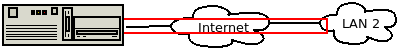
\includegraphics[width=0.9\linewidth]{vpn-host_to_network.png}
	\caption{Host to Network VPN}
	\label{fig:VPNHostToNetwork}
	\end{figure}
\item[host-to-internet] maskeer je IP-adres op Internet door gebruik te maken van een VPN server op Internet waarbij al je verkeer lijkt te komen van deze VPN-server en je dus bijna niet meer te traceren bent. Zie \ref{fig:HostToInternet}
	\begin{figure}[h]
	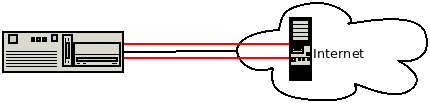
\includegraphics[width=0.9\linewidth]{vpn-host_to_internet.png}
	\caption{Host to Internet VPN}
	\label{fig:VPNHostToInternet}
	\end{figure}
\end{description}

De verschillende soorten VPNs op basis van de techniek:
\begin{description}
\item[Datalink-Layer-VPN] Een VPN die gebruikt maakt van technieken op OSI-layer 2. Voor de erboven gelegen protocolen zou de techniek transparant moeten zijn.
\item[Network-Layer-VPN] Een VPN die gebruikt maakt van technieken op OSI-layer 3. Veelal een vervanging of aanvulling op het IP-protocol.
\item[Transport-Layer-VPN] Een VPN die gebruikt maar van technieken op de transport en applicatie layer om een VPN op te bouwen.
\end{description}
